\documentclass[a4paper]{article}

\newcommand{\docTitle}{Künstliche Inteligenz und Maschineslles Lernen}

\usepackage{datetime2}  % for dates
\usepackage[utf8]{inputenc} % UTF-8 input encoding
\usepackage[T1]{fontenc} % fixes \textquotedbl with pdflatex/OT1
\usepackage{textcomp}   % additional text symbols for typewriter/upquote
\usepackage{xcolor}     % for gray color
\usepackage{listings}
\usepackage{marginnote} % for horizontal margin notes
\usepackage{parskip}
\usepackage{amsmath,amssymb,mathtools}
\usepackage{everypage}
\usepackage{fancyhdr}
\usepackage{amsfonts}   % Mengen and natural numbers
\usepackage{enumerate}  % Custom Enumerations
\usepackage[inline]{enumitem}   % List spacing and labels
\usepackage{multicol}   % Multiple Columns
\usepackage{tabularx}

\usepackage{hyperref}   % Links
\hypersetup{
    pdftitle={\docTitle},
    pdfauthor={Moritz Köhler},
    pdfkeywords={DHBW, Hochschule},
    colorlinks=true,
    linkcolor=black,
    filecolor=magenta,
    urlcolor=cyan
}

% -------
% Images
% -------

\usepackage{import}
\usepackage{xifthen}
\usepackage{pdfpages}
\usepackage{tikz}
\usetikzlibrary{arrows.meta, positioning}

\newcommand{\incfig}[1]{%
    \def\svgwidth{\columnwidth}
    \import{./fig/}{#1.pdf_tex}
}

% ---------------------------------
% Vertical Side note (Bottom Left)
% ---------------------------------

\newcommand{\verticaldocinfo}{%
  \rotatebox{90}{\tiny\color{gray}\texttt{\DTMtoday\_\docTitle\_\jobname}}%
}

\AddEverypageHook{
  \put(-40pt,-650pt){\verticaldocinfo}%
}

% ---------------
% Math Shortcuts
% ---------------

% Number sets
\newcommand{\R}{\mathbb{R}}
\newcommand{\N}{\mathbb{N}}
\newcommand{\Z}{\mathbb{Z}}
\newcommand{\Q}{\mathbb{Q}}
\newcommand{\C}{\mathbb{C}}

% Vectors and matrices
\newcommand{\vect}[1]{\mathbf{#1}}
\newcommand{\mat}[1]{\mathbf{#1}}

% Derivatives
\newcommand{\dd}{\mathrm{d}}
\newcommand{\dpartial}[2]{\frac{\partial #1}{\partial #2}}
\newcommand{\ddt}{\frac{\dd}{\dd t}}

% Norms and absolute values
\newcommand{\norm}[1]{\left\lVert #1 \right\rVert}
\newcommand{\abs}[1]{\left\lvert #1 \right\rvert}

% Probability & Statistics
\newcommand{\E}{\mathbb{E}}
\newcommand{\Var}{\mathrm{Var}}
\newcommand{\Prob}{\mathbb{P}}

% Fields and Algebras
\newcommand{\K}{\mathbb{K}}
\newcommand{\F}{\mathbb{F}}

% Set Operations
\newcommand{\compl}[1]{#1^{\mathrm{c}}}

% Matrix and Vector Operations
\newcommand{\T}{^{\top}}
\newcommand{\inv}{^{-1}}
\newcommand{\conj}[1]{\overline{#1}}

% -------------------
% Main lecture macro 
% -------------------

\newcommand{\lecture}[1]{%
  \protect\marginnote{\protect\tiny\protect\color{gray}#1}
}

% -----------------------------
% Command for box with heading
% -----------------------------

\fboxsep2mm
\newcommand{\know}[2]{
    \noindent\fbox{
        \parbox{\textwidth-21pt}{

            \textbf{#1:}
            \vspace{0.125cm}

            #2
        }
    }
}

% -------------------
% Listings Languages
% -------------------

% Shared defaults for code listings
\lstset{
    basicstyle=\ttfamily\small,
    keywordstyle=\color{blue}\bfseries,
    commentstyle=\color{gray},
    stringstyle=\color{teal},
    numberstyle=\tiny\color{gray},
    numbers=left,
    stepnumber=1,
    numbersep=8pt,
    showstringspaces=false,
    frame=single,
    breaklines=true,
    tabsize=4,
    keepspaces=false,
    columns=flexible,
    upquote=true,
    extendedchars=false % disable extended char handling to avoid UTF-8 conflicts
}

% SQL syntax highlighting
\lstdefinelanguage{SQL}{
    morekeywords={SELECT,FROM,WHERE,INSERT,INTO,VALUES,UPDATE,SET,DELETE,CREATE,TABLE,PRIMARY,KEY,NOT,NULL,AND,OR,JOIN,LEFT,RIGHT,INNER,ON,AS,ORDER,BY,GROUP,HAVING,LIMIT},
    sensitive=false,
    morecomment=[l]{--},
    morestring=[b]'
}

% JSON syntax highlighting
\lstdefinelanguage{json}{
    morestring=[b]",
    stringstyle=\color{teal},
    comment=[l]{//},
    morecomment=[s]{/*}{*/},
        morekeywords={true,false,null},
    literate=
     *{0}{{{\color{blue}0}}}{1}
      {1}{{{\color{blue}1}}}{1}
      {2}{{{\color{blue}2}}}{1}
      {3}{{{\color{blue}3}}}{1}
      {4}{{{\color{blue}4}}}{1}
      {5}{{{\color{blue}5}}}{1}
      {6}{{{\color{blue}6}}}{1}
      {7}{{{\color{blue}7}}}{1}
      {8}{{{\color{blue}8}}}{1}
      {9}{{{\color{blue}9}}}{1}
            {:}{{{\color{black}:}}}{1}
            {,}{{{\color{black},}}}{1},
    showstringspaces=false
}

% Language specific styles
\lstdefinestyle{javastyle}{
    language=Java,
    basicstyle=\ttfamily\small,
    keywordstyle=\color{blue}\bfseries,
    commentstyle=\color{gray},
    stringstyle=\color{teal},
    numberstyle=\tiny\color{gray},
    numbers=left,
    stepnumber=1,
    numbersep=8pt,
    showstringspaces=false,
    frame=single,
    breaklines=true,
    tabsize=4,
    keepspaces=true,
    columns=fullflexible,
    upquote=true
}

\lstdefinestyle{sqlstyle}{
    language=SQL,
    basicstyle=\ttfamily\small,
    keywordstyle=\color{blue}\bfseries,
    commentstyle=\color{gray},
    stringstyle=\color{teal},
    numberstyle=\tiny\color{gray},
    numbers=left,
    stepnumber=1,
    numbersep=8pt,
    showstringspaces=false,
    frame=single,
    breaklines=true,
    tabsize=4,
    keepspaces=true,
    columns=fullflexible,
    upquote=true
}

\lstdefinestyle{pythonstyle}{
    language=Python,
    basicstyle=\ttfamily\small,
    keywordstyle=\color{blue}\bfseries,
    commentstyle=\color{gray},
    stringstyle=\color{teal},
    numberstyle=\tiny\color{gray},
    numbers=left,
    stepnumber=1,
    numbersep=8pt,
    showstringspaces=false,
    frame=single,
    breaklines=true,
    tabsize=4,
    keepspaces=true,
    columns=fullflexible,
    upquote=true
}

\lstdefinestyle{cstyle}{
    language=C,
    basicstyle=\ttfamily\small,
    keywordstyle=\color{blue}\bfseries,
    commentstyle=\color{gray},
    stringstyle=\color{teal},
    numberstyle=\tiny\color{gray},
    numbers=left,
    stepnumber=1,
    numbersep=8pt,
    showstringspaces=false,
    frame=single,
    breaklines=true,
    tabsize=4,
    keepspaces=true,
    columns=fullflexible,
    upquote=true
}

\lstdefinestyle{bashstyle}{
    language=bash,
    basicstyle=\ttfamily\small,
    keywordstyle=\color{blue}\bfseries,
    commentstyle=\color{gray},
    stringstyle=\color{teal},
    numberstyle=\tiny\color{gray},
    numbers=left,
    stepnumber=1,
    numbersep=8pt,
    showstringspaces=false,
    frame=single,
    breaklines=true,
    tabsize=4,
    keepspaces=true,
    columns=fullflexible,
    upquote=true
}

\lstdefinestyle{jsonstyle}{
    language=json,
    basicstyle=\ttfamily\small,
    keywordstyle=\color{blue}\bfseries,
    commentstyle=\color{gray},
    stringstyle=\color{teal},
    numberstyle=\tiny\color{gray},
    numbers=left,
    stepnumber=1,
    numbersep=8pt,
    showstringspaces=false,
    frame=single,
    breaklines=true,
    tabsize=4,
    keepspaces=true,
    columns=fullflexible,
    upquote=true
}

% Default listing style
\lstset{language={}}

\title{\docTitle}
\author{Moritz}
\date{\today}

\begin{document}
\maketitle
\tableofcontents

\lecture{2026-09-29}

\section{Logiksysteme}

\subsection{Begriffe}

Eine Formel ist \dots

\begin{itemize}
    \item eine Tautologie
    \item erfüllbar
    \item allgemeingültig
    \item wiederspruchsvoll
    \item logisch Folgerung aus einer Menge M
\end{itemize}

Was ist eigentlich \dots

\begin{itemize}
    \item das Deduktionstheorem
    \item die Modus-Ponens-Regel
    \item ein Deduktives System
    \item ein Axiom
    \item ein Theorem
    \item ein Term
    \item eine Formel
    \item eine Interpretation
    \item ein Modell
\end{itemize}

Wann ist ein Deduktives System \dots

\begin{itemize}
    \item vollständig?
    \item korrekt?
\end{itemize}

Was ist eigentlich \dots

\begin{itemize}
    \item konjunktive Normalform
    \item disjunktive Normalform
    \item pränexe Normalform
    \item Skolem-Normalform
\end{itemize}

\subsection{Resolution}

Wir haben einige Übungen an der Prädikatenlogik gemacht.

Beweisen Sie: 

\marginpar{Hausaufgabe}

\begin{equation}
    \neg\exists y \forall z[p(z,y) \iff \neg\exists x[p(z,x) \land p(x,z)]] 
\end{equation}

ist allgemeingültig. Die Lösung dzu gibt es evtl. auf Moodle.

Spannende Übung: Minesweeper Prädikat isSafe(x, y) als Logik ausdrücken.

Lösung:

\begin{align*}
    & \operatorname{isSafe}(x, y)\\
    & \operatorname{isMine}(x, y) \quad \text{(hier ist eine Mine)}\\
    \forall x,y\; & \operatorname{isMine}(x, y) \implies \neg\operatorname{isSafe}(x, y)\\
    \forall x,y\; & \operatorname{allMinesFound}(x, y) \implies
        \forall u,v\; \bigl((\operatorname{Neighbor}(x, y, u, v) \land
        \operatorname{unknown}(u, v)) \implies \operatorname{isSafe}(u, v)\bigr)\\
    \forall x,y\; & \bigl(\#\operatorname{mines}(x, y) =
        \operatorname{label}(x, y)\bigr) \implies \operatorname{allMinesFound}(x, y)
\end{align*}

\begin{align*}
    \text{Funktionen:} & \#\operatorname{mines}(x, y)\\
    & \operatorname{label}(x, y)
\end{align*}


\subsection{Deduktive Datenbanken}

\subsection{Vor und Nachteile}

\begin{tabularx}{\textwidth}{XXX}
    Repräsentationsform & 
    Ausdruckskraft & 
    Kalkülmäßige Verarbeitung \\
    \hline
    Aussagenlogik & 
    Schwach, nur Information kodiert darstellbar &
    Gut, gewisse Komplexitätsprobleme \\
    Hornlogik & 
    Für viele Anwendungen hinreichend & 
    Prinzipiell gut, verstärkt Komplexitätsprobleme \\
    Prädikatenlogik 1. Stufe &
    Kann die meisten Situationen zumindest fragmentarisch darstellen & 
    In Balance mit der Ausdruckskraft\\
    Höhere Prädikatenlogik & 
    Umfassend & 
    Sehr schlecht \\
\end{tabularx}

\subsection{Modellierung von Zeit}

Die Zeit kann Verzweigungen sein, ob ein Ereignis stattfindet oder nicht. Also Zug verpassen oder bekommen. 

Allen's Zeitlogik: \href{https://de.wikipedia.org/wiki/Allen-Kalk%C3%BCl}{Wikipedia}

Statt den Inversen Funktionen können auch einfach die Reihenfolge der Parameter getauscht werden.

Wir können auch unsere Inferenz in einer 13x13 Lookup-Tabelle speichern.

\begin{center}
    \includegraphics[
        page=20,
        width=0.9\textwidth
    ]{doc/DHBW_KI_003_Logik_2022.pdf}
\end{center}

\lecture{2026-10-06}

Hinweise:

\begin{itemize}
    \item Globale Konsistenzprüfung ist NP-Hard
    \item Konsistenz kann nur als lokale Konsistenz garantiert werden (d.h. in einem drei-knotigen Teilnetz)
\end{itemize}

Für die Berechnung in einem Teilnetz muss bei Rückwertsgehen der Kanten, die Inversen der Zeitlichen Operatoren genommen werden.

\begin{equation}
    P(X, Y) = \land (p(R,S) \mid R\in X, S\in Y)
\end{equation}

\begin{center}
    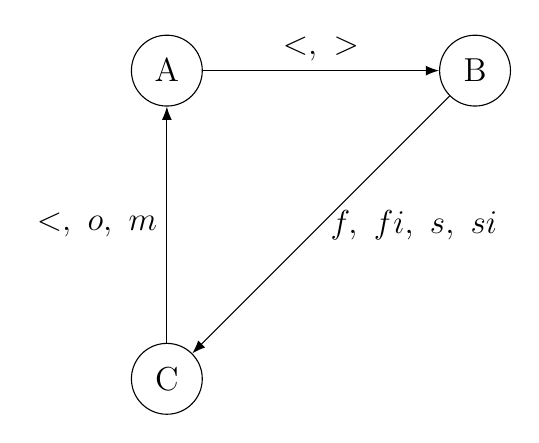
\begin{tikzpicture}[
        >=Latex,
        node distance=3cm,
        every node/.style={font=\large},
        state/.style={circle, draw, minimum size=9mm}
    ]
        \node[state] (A) {A};
        \node[state, right=of A] (B) {B};
        \node[state, below=of A] (C) {C};

        \draw[->] (A) -- node[above] {$<,\ >$} (B);
        \draw[->] (B) -- node[right] {$f,\ fi,\ s,\ si$} (C);
        \draw[->] (C) -- node[left] {$<,\ o,\ m$} (A);
    \end{tikzpicture}
\end{center}

\begin{align*}
    P(\{fi, f, si, s\}, \{>, <\}) = &\{<, o, m, di, fi, >, oi, mi, si\}&\\
    &\{<, o, m, di, fi, >, oi, mi, si\} &\land \overrightarrow{CA} \neq \emptyset ?\\
    &P(\{<, oi, mi\}, \{fi,f, si, s\}) &\land \overrightarrow{AB} \neq \emptyset ?\\
    &P(\{>, <\}, \{<, oi, mi\}) &\land \overrightarrow{BC} \neq \emptyset ?
\end{align*}

Diese Netze und Konsistenzprüfung können für z.B. Produktionsplanung genutzt werden.

\subsection{Modale Logik}

Hier gibt es noch 2 weitere neue logische Symbole:

\begin{align*}
    \Box \Phi&: \Phi \text{gilt "notwendigerweise}\\
    \lozenge \Phi&: \Phi \text{gilt "möglicherweise}
\end{align*}

\subsection{Schlussregeln}

Deduktiver Schluss. Wenn $A$ gilt und $A\implies B$, dann gilt auch $B$. Immer gültig, sicheres Schließen (apodiktisch)

Induktiver Schluss. Wenn für $n$ Beispiele gilt, Schließen wir auf die Allgemeinheit. Nicht unbedingt gültig, Verallgemeinerung (dialektisch). So lernt Maschine Learning.

Abduktiver Schluss. Wenn $B$ gilt und $A\implies B$, dann gilt $A$. Hypothetisch, von Symptom auf Ursache schließen (rhetorisch)

\end{document}